\documentclass[twocolumn]{article}
\usepackage{amsmath}
\usepackage{graphicx}
\usepackage{hyperref}
\title{Factoring with $n+2$ clean qubits and $n-1$ dirty qubits}
\author{Craig Gidney}

\begin{document}
\maketitle

\begin{abstract}
\em
We present asymptotically size-efficient reversible classical circuits for performing various arithmetic operations aided by ancilla in an unknown state.
We improve the number of qubits needed to factor an $n$-bit number with Shor's algorithm \cite{Shor1999} from $2n+2$ clean qubits \cite{takahashi2006, haner2016} to $2n+1$ qubits, $n-1$ of which can be an unknown state, without increasing the asymptotic size or depth of the circuit.
\end{abstract}

\section{Introduction}

When constructing quantum circuits, or classical reversible circuits, an important resource is the number of available ancilla.
An ancilla is an extra bit or qubit available for use by a circuit as temporary workspace.
Ancilla may be initialized to a known state (``clean bit"), or be given to the circuit in an unknown state (``dirty bit") that must be restored before the circuit finishes.
Clean bits are more valuable, allowing for simpler and more compact circuit constructions, but dirty bits are more plentiful, since any temporarily unused bit is a borrowable dirty bit.

Because one part of a circuit can borrow dirty bits from another part of the same circuit, circuit constructions that require only dirty bits are easier to apply under tight space constraints, or on circuit topologies where other ancilla are too far away to be acquired quickly.
When attempting to reduce the number of bits or qubits required by a circuit, converting clean ancilla to dirty ancilla makes a useful intermediate goal.
In this paper, at great cost to the constant factors in the gate count and depth, we reduce the number of qubits required to perform period finding from $2n+2$ clean qubits \cite{takahashi2006, haner2016} to $n+2$ clean qubits and $n-1$ dirty qubits without increasing the asymptotic costs.

Our paper is structured as follows.
The introduction describes the various sections and also itself for no discernible reason.
In section \ref{sec:construct} we describe all the circuit constructions needed to reduce period finding into constant-sized gates, while tracking the number of required dirty ancilla.
Then, in section \ref{sec:costs}, we discuss the novelty and comparative costs of the presented circuit constructions.
Finally, section \ref{sec:conclusion} concludes and summarizes.

All constructions assume a 2s-complement representation of integers.
Multi-qubit arithmetic operations always have the least significant bit towards the top.
All dirty qubit counts are for classical Toffoli-based constructions, without using the quantum ancilla bootstrap trick noted in figure \ref{fig:bootstrap-ancilla}.
For clarity, circuit diagrams will divide operations into separate input and output parts, with inputs shaded gray, when applicable.
For completeness, even when the period finding reduction doesn't produce a controlled version of an operation, we always provide controllable constructions that scale linearly with the number of controls.


\section{Period Finding into Toffolis} \label{sec:construct}

\subsection{Period Finding}

A high-level circuit for period finding, the core quantum subroutine of Shor's quantum factoring algorithm \cite{Shor1999}, is shown in figure \ref{fig:period-finding}.
The circuit starts by preparing a uniform superposition $|\psi_0\rangle = \sqrt{2^{-n}} \sum_{k=0}^{2^n} |k\rangle$, then uses the $\times B^A {\pmod R}$ operation to separate that superposition into equivalence classes modulo the unknown period $p$ of that operation.
That is to say, w.l.o.g. the state ends up being $|\psi_{1,x}\rangle = \sqrt{2^{-n}/p} \sum_{k=0}^{2^n/p} |pk + x \rangle$ for some $x$.
The circuit then applies an inverse Fourier transform and samples the output.
Using a classical continued fraction algorithm, the sample can be used to estimate the period.

Because period-finding measures all qubits immediately after performing a QFT, most of the transformed qubits can be measured earlier than shown.
In fact, each qubit can be measured so early that the next qubit needed for the QFT does not even need to be initialized yet!
Only one of the qubits in the phase-estimation register needs to be present at a time, and so the phase register can be reduced to a single repeatedly-used qubit \cite{beauregard2003}.
Figure \ref{fig:period-finding-solo-phase-qubit} shows a period-finding circuit with this property.

The period-finding circuit in figure \ref{fig:period-finding-solo-phase-qubit} is our high-level starting point.
It uses (a) controlled modular multiplication, (b) measurement, (c) X-axis rotations classically parametrized by previous measurements, and (d) qubit resets.
The only non-trivial operation is (a), the controlled modular multiplication of an $n$-qubit register (requiring $n-1$ dirty ancilla and 1 clean ancilla using our constructions).

We perform modular multiplication with multiply-accumulates and a second clean register as in \cite{beauregard2003}.
However, to allow the second register to be mostly dirty, we note that each modular multiplication on the first register causes an inverse and negated multiplication on the second register.
We will refer to this combined operation as a ``bimultiply".

Note that we must preserve the state of the second register, but bimultiplication trashes that state with many multiplications by unknown constants.
However, because the first register is initialized to $|1\rangle$ and gets multiplied by constants inverse to the ones trashing the second register, we can fix the second register by measuring the first register and using its value to perform a clean-up bimultiplication after the usual end of the circuit.
Figure \ref{fig:period-finding-solo-phase-qubit-explicit-dirty-register} shows this construction.

Our modular circuit constructions do not guarantee that out-of-range values (i.e. values not below the modulus $R$) are well behaved.
If the second register contained a value larger than $R$, it would end up trashed despite the final clean-up operation.
To avoid this problem, we require that the registers have minimal size $n = \lceil \lg_2(R-1) \rceil$ and that the second register's most-significant-bit (MSB) be a clean qubit initialized to zero.

\begin{figure}
  \centering
  \makebox[\linewidth]{
    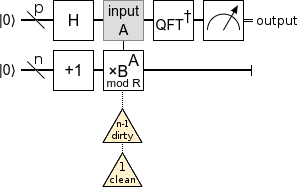
\includegraphics[width=\linewidth]{assets/shor-period-finding.png}
  }
  \caption{\em
	High-level period finding circuit \cite{Shor1999}.
	$R$ is the modulus being queried, $B$ is a randomly chosen base, $n$ is the number of bits needed to store $R$, and $p \in \Theta(n)$ controls the precision of the phase estimation step.
    The triangles indicate how many ancilla are needed ``behind the scenes", by our constructions, to perform an operation.
	Recovering the period requires classical post-processing of the sampled output.
  }
  \label{fig:period-finding}
\end{figure}

\begin{figure*}
  \centering
  \makebox[\linewidth]{
    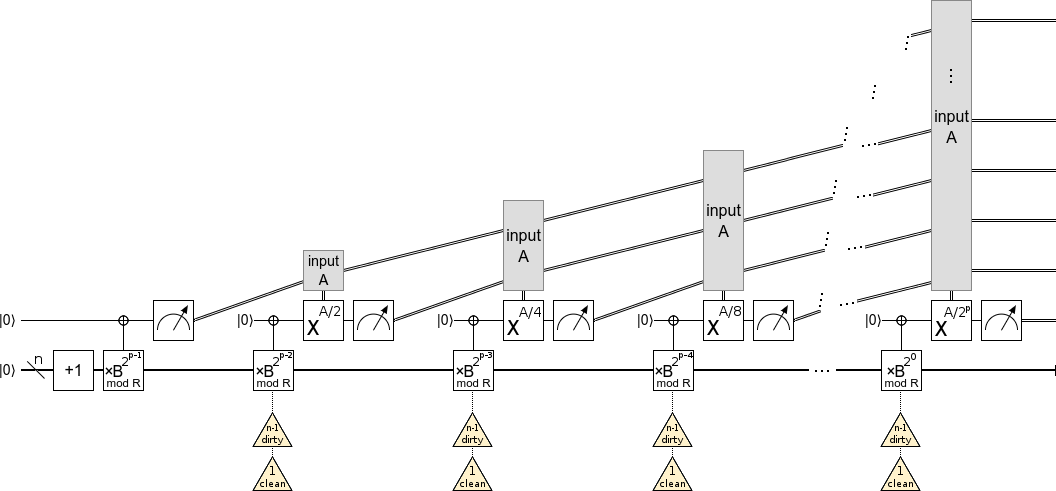
\includegraphics[width=\linewidth]{assets/shor-period-finding-solo-phase-qubit.png}
  }
  \caption{\em
	Period finding with a single phase-estimation qubit \cite{beauregard2003}.
	The small oplus' ({\tiny $\oplus$}) are ``X-axis controls".
	An X-axis control is equivalent to a normal control, but with a Hadamard gate applied before and after.
	It conditions on the state $\frac{1}{\sqrt 2}|0\rangle - \frac{1}{\sqrt 2}|1\rangle$ instead of on the state $|1\rangle$.
  }
  \label{fig:period-finding-solo-phase-qubit}
\end{figure*}

\begin{figure*}
  \centering
  \makebox[\linewidth]{
    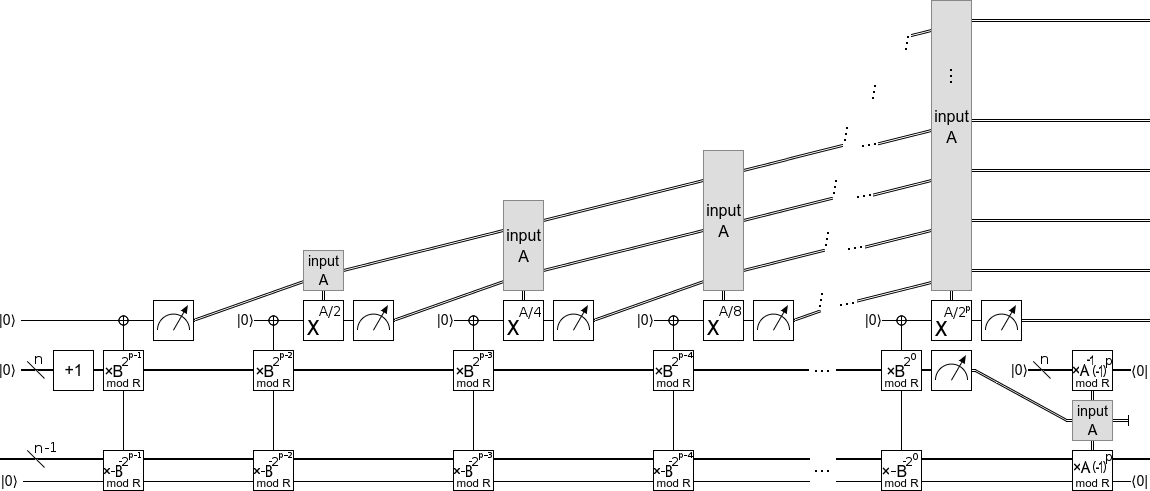
\includegraphics[width=\linewidth]{assets/shor-period-finding-solo-phase-qubit-double-register.png}
  }
  \caption{\em
	Period finding with a single phase-estimation qubit and paired inverse multiplications.
	The terminating bra $\langle 0 |$ indicates that the bottom wire will always end up in the state $|0\rangle$, without post-selection.
  }
  \label{fig:period-finding-solo-phase-qubit-explicit-dirty-register}
\end{figure*}


\subsection{Modular Bimultiplication}

As in \cite{beauregard2003}, we perform controlled modular multiplication with a second register and modular scaled-accumulate operations.
However, because the second register is dirty, we need three scaled-accumulates instead of the usual two.

As with all other modular arithmetic circuits in this paper, we make no guarantees about the circuit's behavior when either of the input registers is out of range (i.e. have values not below $R$).

Suppose that the two registers start in the state $(a, b)$, working modulo $R$.
By scale-adding the first register times $K$ into the second register, the system advances to $(a, b+aK)$.
Then a scale-subtract times $K^{-1}$ out of the first register puts the system into the state $(a-bK^{-1}-aKK^{-1}, b+aK)$, which is just $(-bK^{-1}, b+aK)$.
Next, we cancel the $b$ term in the second register by scale-adding the first register times $K$ into it again, leaving $(-bK^{-1}, b+aK-bK^{-1} \cdot K)$ which is simply $(-bK^{-1}, aK)$.
Finally, we swap to $(aK, bK^{-1})$.
The overall effect is to multiply the first register by $K$ and the second register by $-K^{-1}$, as desired.
See figure \ref{fig:controlled-modular-multiply} for the circuit diagram.

In the case where $K$ has no multiplicative inverse modulo $R$, this construction will not work (it would define an invalid irreversible operation).
However, that would mean $K$ is a factor of $R$, a case that the very lucky user can check for and handle classically before invoking a quantum period finding circuit.

\begin{figure}
  \centering
  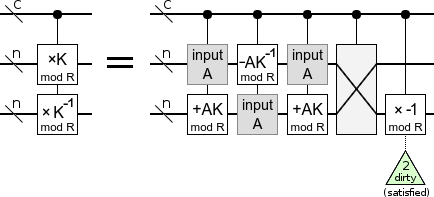
\includegraphics[width=\linewidth]{assets/controlled-modular-multiply.png}
  \caption{\em
    Controlled modular bimultiplication, with a constant multiplier $K$, using three modular scaled-accumulates and a swap.
    $K$ must have a multiplicative inverse modulo $R$.
    Uses no ancilla, $O(c + n^2 \lg n)$ gates, and $O(c + n^2)$ depth where $c$ is the number of controls and $n$ is the register size.
  }
  \label{fig:controlled-modular-multiply}
\end{figure}


\subsection{Modular Scaled-Accumulation}

To perform scaled-accumulate, we use a shift-and-add approach similar to \cite{beauregard2003}.
We right-shift (i.e. divide by $2 {\pmod R}$) the target register $n-1$ times, then begin iteratively left-shifting (i.e. multiplying it by 2) and adding $K$ into the target.
We condition the first modular addition on the most significant bit of the input, the second addition on the next most significant bit, and so forth.
(The more significant bits go first because their effects must be hit by more left-shifts.)
See figure \ref{fig:controlled-modular-scale-accumulate}.

The conditional offset and modular doubling operations need one dirty bit, but for non-trivial $n$ there are more than enough unused bits available to borrow, so the circuit as a whole doesn't require any dirty bits.

Note that the modular doublings require $R$ to be odd, since otherwise the operation would be irreversible and non-unitary.
However, given that in the intended use case $R$ is a number to be factored, it is reasonable to require callers to have factored out multiples of two beforehand.

As will all circuits presented in this paper (except the period-finding circuit), we define the construction of the inverse operation to be the same circuit but run in reverse order with each sub-operation inverted.
A decrement is just a reversed increment, a division is just a reversed multiplication, etc.

\begin{figure}
  \centering
  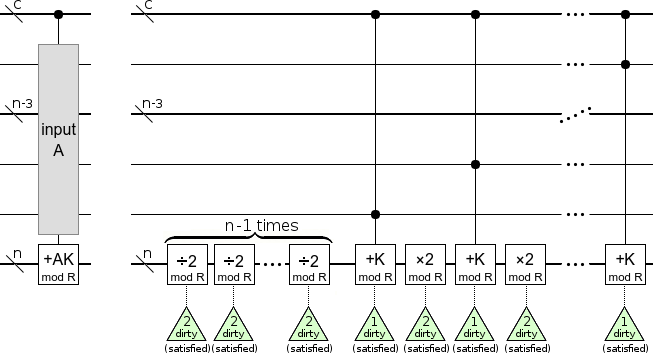
\includegraphics[width=\linewidth]{assets/controlled-modular-multiply-accumulate.png}
  \caption{\em
    Reducing a controlled modular scale-accumulate, with a constant multiplier $K$, into the modular equivalent of shift-and-add.
    Requires the modulus $R$ to be odd.
    Uses no ancilla, $O(c + n^2 \lg n)$ gates, and $O(c + n^2)$ depth where $c$ is the number of controls and $n$ is the register size.
  }
  \label{fig:controlled-modular-scale-accumulate}
\end{figure}


\subsection{Modular Doubling}

To multiply a register by 2 modulo an odd $R$, we use controlled offsets and nots to shift the top half of the input space until it starts on the MSB boundary.
Once that's done, a left-rotate completes the operation by turning the MSB into the LSB (converting the alignment into interleaving).
See figure \ref{fig:modular-double}.

\begin{figure}
  \centering
  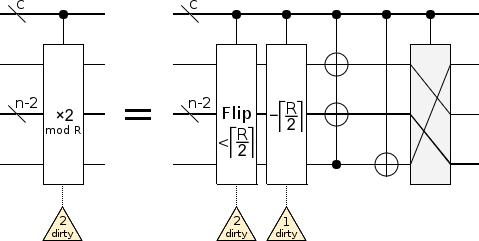
\includegraphics[width=\linewidth]{assets/controlled-modular-double.png}
  \caption{\em
    Controlled modular doubling in $O(c + n \lg n)$ gates, $O(c + n)$ depth, with 2 dirty ancilla.
    $R$ must be odd.
    Uses 1 dirty ancilla, $O(c + n \lg n)$ gates, and $O(c + n)$ depth where $c$ is the number of controls and $n$ is the register size.
  }
  \label{fig:modular-double}
\end{figure}


\subsection{Modular Addition / Offset}

As shown in figure \ref{fig:mod-add-from-pivot-flip-bars}, a modular addition is three pivot-flips (see section \ref{sec:pivot-flips}).
To add $A$ into a register modulo $R$, perform pivot-flips with the pivot at $R-A$, then $R$, then $A$.
See figure \ref{fig:controlled-modular-add} for the circuit.

Interestingly, modular addition can use its own controls as dirty bits that would otherwise be required.
For modular offset (i.e. adding a compile-time constant into a register), the two dirty bits are required whether or not the operation is controlled.
See figure \ref{fig:controlled-modular-offset}.

\begin{figure}
  \centering
  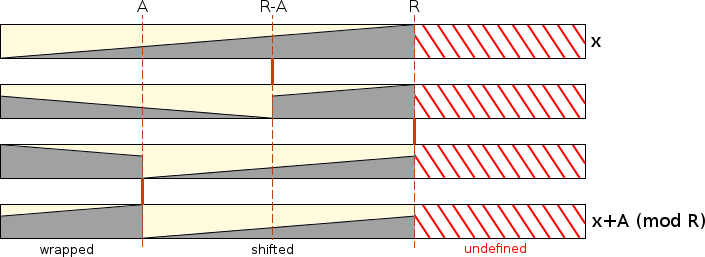
\includegraphics[width=\linewidth]{assets/mod-add-from-pivot-flip-bars.png}
  \caption{\em
     Modular addition of $A \pmod{R}$ can be done with three pivot flips.
     One at $R-A$, then one at $R$, then one at $A$.
     Requires $A \leq R$.
   }
  \label{fig:mod-add-from-pivot-flip-bars}
\end{figure}

\begin{figure}
  \centering
  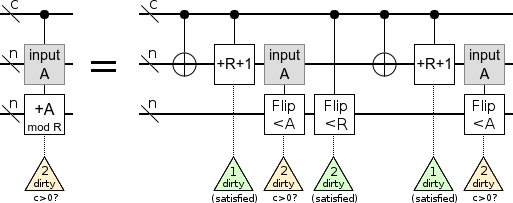
\includegraphics[width=\linewidth]{assets/controlled-modular-addition.png}
  \caption{\em
    Controlled modular addition construction based on pivot-flips.
    Uses $2-c$ dirty ancilla, $O(c + n \lg n)$ gates, and $O(c + n)$ depth where $c$ is the number of controls and $n$ is the register size.
  }
  \label{fig:controlled-modular-add}
\end{figure}

\begin{figure}
  \centering
  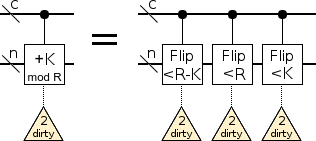
\includegraphics[width=\linewidth]{assets/controlled-modular-offset.png}
  \caption{\em
    Controlled modular offset construction based on pivot-flips.
    Uses $2$ dirty ancilla, $O(c + n \lg n)$ gates, and $O(c + n)$ depth where $c$ is the number of controls and $n$ is the register size.
  }
  \label{fig:controlled-modular-offset}
\end{figure}


\subsection{Pivot-Flips} \label{sec:pivot-flips}

We implemented both modular doubling and modular offset/addition in terms of a non-standard operation we call a ``pivot-flip".
A pivot-flip is an operation that reverses the order of states less than a given pivot value, without affecting other states.
For example, a pivot-flip with the pivot equal to 4 would swap $|0\rangle$ and $|3\rangle$, swap $|1\rangle$ and $|2\rangle$, and leave all other states untouched.

The exact permutation performed by a pivot-flip with pivot equal to $A$ is:

$$\text{PivotFlip}_A = \sum_{i=0}^{A-1} |A-i-1\rangle \langle i| + \sum_{i=A}^{N-1} |i\rangle \langle i|$$

To perform a pivot-flip efficiently, we use the fact that $x \rightarrow \lnot(x - A)$ nearly does what is required: it flips the range below $A$ but unfortunately also flips the range above-and-including $A$.
However, because $x \rightarrow \lnot(x - A)$ is its own inverse, the operation can be ``toggle-controlled'', where the operation undoes itself unless a controlling qubit is toggled between two applications.
Also, because the operation doesn't change whether a given value is below the pivot, the controlling qubit can be toggled by a comparison of the target against the pivot $A$ even though the target is being operated on.

See figures \ref{fig:controlled-pivot-flip} and \ref{fig:controlled-const-pivot-flip} for the circuit diagrams.
For states that are less than the pivot $A$, the comparison against the pivot keeps toggling the ancilla and exactly one of the controlled subtract-and-inverts will fire.
For other states, the ancilla does not change and so the subtract-and-inverse happens either no times or two times (undoing itself) for a net effect of no effect.

Note that, depending on whether or not the pivot is a compile-time constant or another qubit register, different subtraction constructions are used when reducing further.
This distinction matters because the constant-offset construction uses $O(n \lg n)$ gates \cite{haner2016} instead of the $\Theta(n)$ gates used by enregistered addition \cite{takahashi2005}.

\begin{figure}
  \centering
  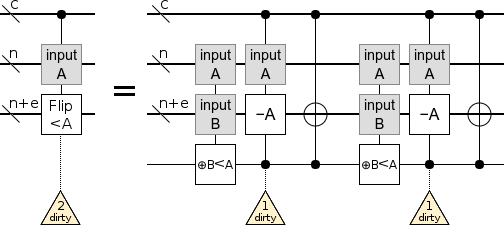
\includegraphics[width=\linewidth]{assets/controlled-pivot-flip.png}
  \caption{\em
    Controlled pivot-flip circuit with an enregistered pivot.
    Uses $2$ dirty ancilla, $O(c + n \lg n)$ gates, and $O(c + n)$ depth where $c$ is the number of controls and $n$ is the register size.
  }
  \label{fig:controlled-pivot-flip}
\end{figure}

\begin{figure}
  \centering
  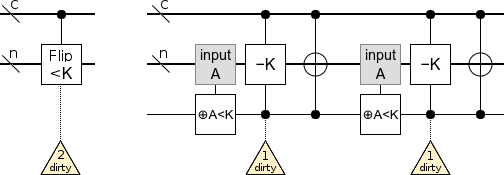
\includegraphics[width=\linewidth]{assets/controlled-const-pivot-flip.png}
  \caption{\em
    Controlled pivot-flip circuit with a constant pivot.
    Uses $2$ dirty ancilla, $O(c + n)$ gates, and $O(c + n)$ depth where $c$ is the number of controls and $n$ is the register size.
  }
  \label{fig:controlled-const-pivot-flip}
\end{figure}


\subsection{Comparison}

Comparison operations toggle a target bit based on the relationship between two input registers.
We implement comparisons as in \cite{takahashi2005}, using an addition followed by a subtraction that is slightly smaller to clear all changes except an overflow signal into the target.
For comparisons against another register this uses $1$ dirty ancilla (if controlled, otherwise no ancilla), $O(c + n)$ gates, and $O(c + n)$ depth.
For comparisons against a constant, the number of gates increases to $O(c + n \lg n)$ and the dirty ancilla is always required.


\subsection{Addition / Offset}

\cite{takahashi2005} provides a reversible adder circuit that uses $O(n)$ gates, $O(n)$ depth, and no ancilla.
We show an equivalent circuit in figure \ref{fig:inlineadder}.
Note that the construction uses the input register as workspace, so it breaks when the input is a compile-time constant or when the target register is larger than the input register.

\begin{figure}
  \centering
  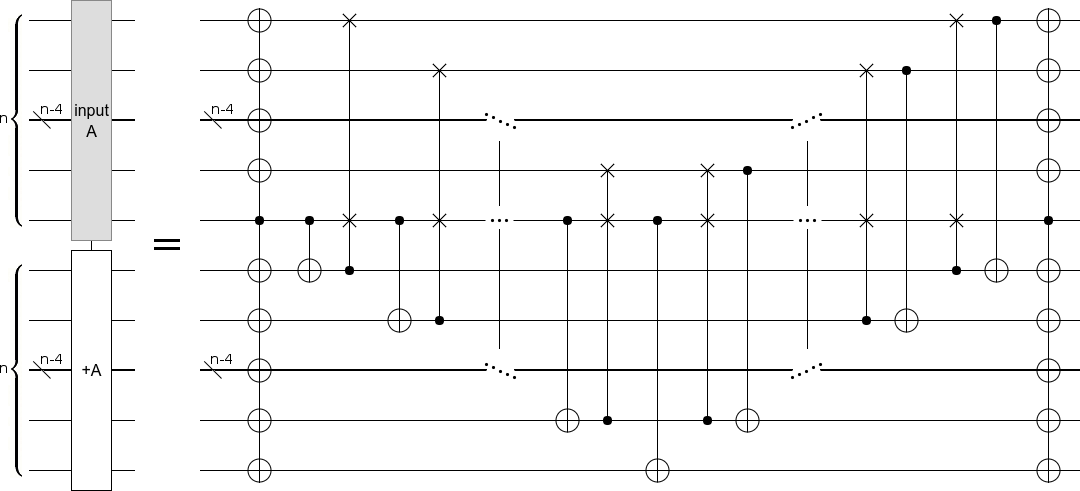
\includegraphics[width=\linewidth]{assets/inline-adder.png}
  \caption{\em Adder for input and target registers of the same size.
  Requires no ancilla, and uses $O(N)$ gates and depth.
  Based on \cite{van2004, takahashi2005}.}
  \label{fig:inlineadder}
\end{figure}

When the value to be added into a register is a compile-time constant (i.e. when applying an offset gate), we use the construction from \cite{haner2016}.
Their offset circuit, shown in figure \ref{fig:offset}, uses $O(n \lg n)$ gates, $O(n)$ depth, and a dirty ancilla.

When the target register is larger than the input register, three tweaks based on increment/decrement gates can be used (instead of increasing the asymptotic costs).
(Note that, to avoid cyclic dependencies, the increment and decrement constructions described in the next subsection will only use the same-register-size adder.)
First, the carry signal is forwarded into the high part of the target register with a controlled increment instead of with a CNOT.
Second, to free the MSB of the input register for use as a dirty ancilla holding the carry signal, we add it into the target ahead of time with a controlled increment.
Finally, when the MSB is on its role as carry signal causes an extra increment of the target.
This extra increment is cancelled with a controlled decrement.
See the circuit diagram in figure \ref{fig:inline-adder-into-large}.

To control addition gates, and offset gates, we do an uncontrolled addition followed by an uncontrolled subtraction bordered by NOT gates that fire when the controls are satisfied.
When the NOT gates don't fire, the subtraction cancels the addition.
When the NOT gates do fire, the subtraction is inverted into an addition and $2 \cdot a$ is added to the target.
To add $a$ instead of $2 \cdot a$ into the target, we temporarily prepend a dirty bit onto the target register.
See \ref{fig:controlled-addition}.

\begin{figure}
  \centering
  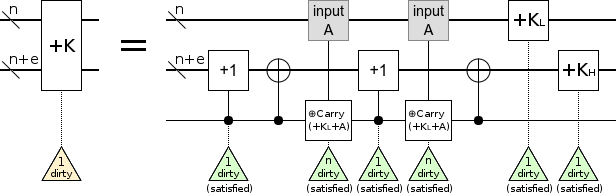
\includegraphics[width=\linewidth]{assets/offset.png}
  \caption{\em
      Offset circuit from \cite{haner2016}.
      Uses $1$ dirty ancilla, $O(n \lg n)$ gates, and $O(n)$ depth (by overlapping the recursive cases).
  }
  \label{fig:offset}
\end{figure}

\begin{figure}
  \centering
  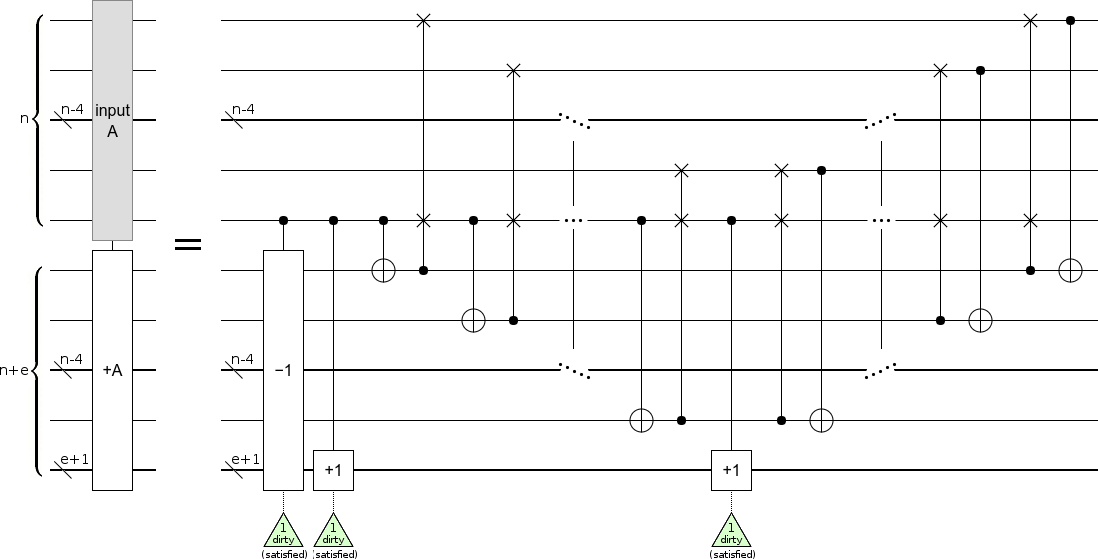
\includegraphics[width=\linewidth]{assets/inline-adder-into-large.png}
  \caption{\em
      Adder with target larger than source, using no ancilla.
      Uses $O(n)$ gates and depth.
      The increment and decrement gates all have at least one free wire to borrow as a dirty ancilla.}
  \label{fig:inline-adder-into-large}
\end{figure}

\begin{figure}
  \centering
  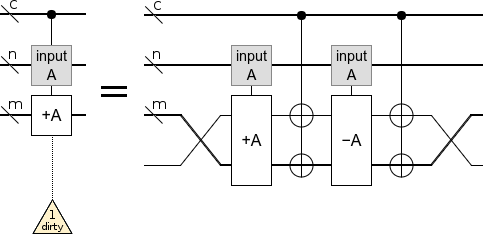
\includegraphics[width=\linewidth]{assets/controlled-addition.png}
  \caption{\em
  	Reducing controlled addition to uncontrolled addition.
  	Uses $O(c + n)$ gates, $O(c + n)$ depth, and a dirty ancilla.
  	When applied to offset gates, uses $O(c + n \lg n)$ gates, $O(n + c)$ depth, and two dirty ancilla.
  }
  \label{fig:controlled-addition}
\end{figure}


\subsection{Increment}

A register can be incremented by subtracting both $x$ and $\neg x = -x-1$ from it, for any $x$.
When $n$ dirty bits are available, $x$ can come from a register defined by those $n$ arbitrary bits, as shown in figure \ref{fig:increment-many-dirty}.

\begin{figure}
  \centering
  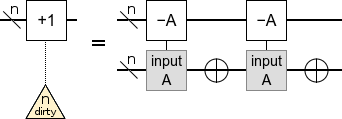
\includegraphics[width=\linewidth]{assets/increment-many-dirty.png}
  \caption{\em Subtracting $x$ and $-x-1$ from a register increments it. Requires $O(N)$ depth, size, and $N$ dirty ancilla.}
  \label{fig:increment-many-dirty}
\end{figure}

To improve from $n$ dirty bits to a single dirty bit, we break the increment operation into two halves.
A high half that is incremented only if all of the bottom bits are on, and a low half that is unconditionally incremented.
The low half can be incremented with the double-subtraction trick by borrowing the high half.
But the double-subtraction trick doesn't work on the high half, because the low half can't be borrowed when it is being used as a control.

To work around not being able to operate on the borrowed bits while using them as a control, start with the double-subtraction trick but change the second subtraction to an addition and conditionally toggle the target bits instead of the input bits.
When the condition isn't satisfied, the addition and subtraction will cancel each other.
When the condition is satisfied, the addition will be inverted into a subtraction, and both the subtraction and addition-turned-subtraction will fire, subtracting the input register from the target register twice.
However, because we are conditioning on the input bits all being on, we know the input must be -1.
Therefore the target was incremented by 2.
To halve the +2 into a +1, prepend a dirty least-significant-bit onto the target register.

Note that, to avoid a cyclic dependency, we must require that the additions and subtractions use input and target registers of the same size.
So the construction described in the previous paragraph only works for odd-sized registers.
For even-sized registers, we simply handle the LSB separately.
Also, we support contorls with another conditional-inversion trick.
See figure \ref{fig:controlled-increment-odd}.

\begin{figure}
  \centering
  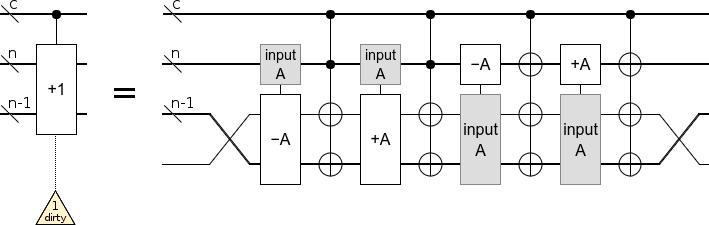
\includegraphics[width=\linewidth]{assets/controlled-increment-odd.png}
  \caption{\em
    Odd-sized controlled increment.
    For the even-sized case, separate the LSB from the rest of the register, increment the rest of the register using the LSB as an extra control, then toggle the LSB.
    Uses $O(c+n)$ gates, $O(c+n)$ depth, and 1 dirty ancilla.
  }
  \label{fig:controlled-increment-odd}
\end{figure}

\begin{figure}
  \centering
  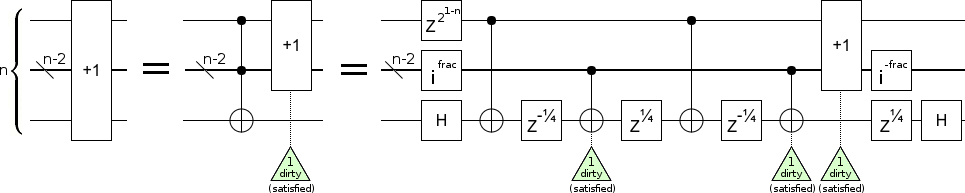
\includegraphics[width=\linewidth]{assets/ancilla-bootstrap.png}
  \caption{\em Bootstrapping a dirty ancilla out of an increment gate using quantum operations.
  The $i^{\text{frac}}$ gate is a ``phase gradient" operation that phases each computational basis state $|v\rangle$ by an amount proportional to $v/2^d$, where $d$ is the size of the register.
  In this case each state is phased by $e^{i \frac{\pi}{2} v/2^d}$.
  The phase gradient is implemented by a column of $Z^{2^{-k}}$ gates, .}
  \label{fig:bootstrap-ancilla}
\end{figure}


\subsection{Bit Swaps, Rotations, and Reversals}

Bit permuting operations can usually be emulated by re-labelling qubits, so they are easy to overlook in circuits.
But some of our circuit diagrams have used controlled bit rotations, requiring actual operations, so we provide the constructions in figures \ref{fig:bit-rotate} and \ref{fig:bit-reverse} for completeness.

\begin{figure}
  \centering
  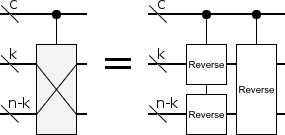
\includegraphics[width=\linewidth]{assets/controlled-bit-rotate.png}
  \caption{\em
    A controlled bit rotation / bit swap is three controlled bit-reverses.
    Uses no ancilla, $O(n+c)$ gates, and $O(n+c)$ depth.
  }
  \label{fig:bit-rotate}
\end{figure}

\begin{figure}
  \centering
  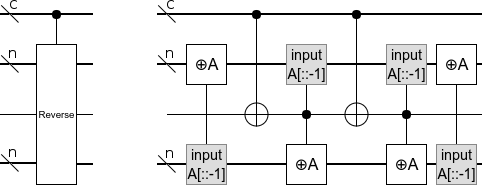
\includegraphics[width=\linewidth]{assets/controlled-reverse.png}
  \caption{\em
    An inline controlled bit order reversal.
    Each XOR operation is a series of independent CNOTs (note that the inputs have opposite endian-ness to the outputs).
    For reversals on an even number of bits, swap the center two bits beforehand then use one of them as the center workspace bit from this construction.
    Uses no ancilla, $O(c + n)$ gates, and $O(c + n)$ depth.
  }
  \label{fig:bit-reverse}
\end{figure}


\subsection{Multi-Nots}

Several of our constructions have used CNOTs with many controls and many targets.
To avoid paying the overhead of $c$ controls for every target, we use one big CNOT to toggle-control all the others.
We then use a dirty ancilla (i.e. one of the other targets) to efficiently reduce the big CNOT into Toffolis.


\section{Overview and Improvements} \label{sec:costs}

In figure \ref{fig:dependencies} we show a dependency graph of the constructions discussed in this paper.
The total cost of period-finding, using the full construction, is $O(n^3 \lg n)$ gates and $O(n^3)$ depth.
We perform $O(n)$ modular multiplications, each of which uses $O(n)$ modular additions and offsets, each of which uses $O(n \lg n)$ gates \cite{haner2016} and $O(n)$ depth.

We tested individual constructions in \href{https://github.com/Strilanc/Quirk}{Quirk} and the full construction down to Toffoli gates in \href{https://github.com/ProjectQ-Framework/ProjectQ}{ProjectQ} \cite{projq2016}. [[[ insert link to code ]]] [[[ maybe make a plot of gate counts vs size? ]]] [[[ definitely need another constant-factor joke ]]]

Our main improvements over previous constructions are 1) the use of pivot-flips for modular addition, 2) the use of bimultiplication for modular multiplication, and 3) the $O(n)$ incrementer requiring only a single dirty ancilla.

Previous modular addition constructions worked by temporarily storing an is-wraparound-needed comparison in a clean ancilla \cite{takahashi2006, haner2016}.
Pivot flips also require ancilla (two, actually), but the ancilla can be dirty and, in the context of period-finding, there's always qubits available to borrow whenever a pivot-flip is needed.
This improvement saves a qubit, reducing the total number of qubits required for period finding from $2n+2$ to $2n+1$.

Previous modular multiplication constructions required a clean ancilla register \cite{haner2016}, where any garbage in the ancilla register would have infected the target register and trashed it.
We deal with the trash with an extra multiply-accumulate per modular multiplication, and cancel the overall effects on the ancilla register with a clean-up multiplication informed by measuring the main register at the end of the circuit.
This improvement allows $n-1$ of the qubits in the ancilla register to be dirty (only the MSB must be zero; to ensure the register's value is in range).

Previous published incrementers (not counting an unpublished version of our construction \cite{gidney2015} cited by \cite{haner2016}) required either $O(n^2)$ gates or $O(n)$ ancilla \cite{draper2000, barenco1995}.
Our classical incrementer constructions use $O(n)$ gates and a single dirty ancilla.
Note that, for classical reversible computation, 1 dirty ancilla is optimal.
The parity of the permutation performed by an increment operation is odd, but the parity of the permutation performed by any classical gate that doesn't cover the entire circuit is even.
With quantum operations, we achieve zero ancilla and $O(n)$ gates (see figure \ref{fig:bootstrap-ancilla}).

\begin{figure}
  \centering
  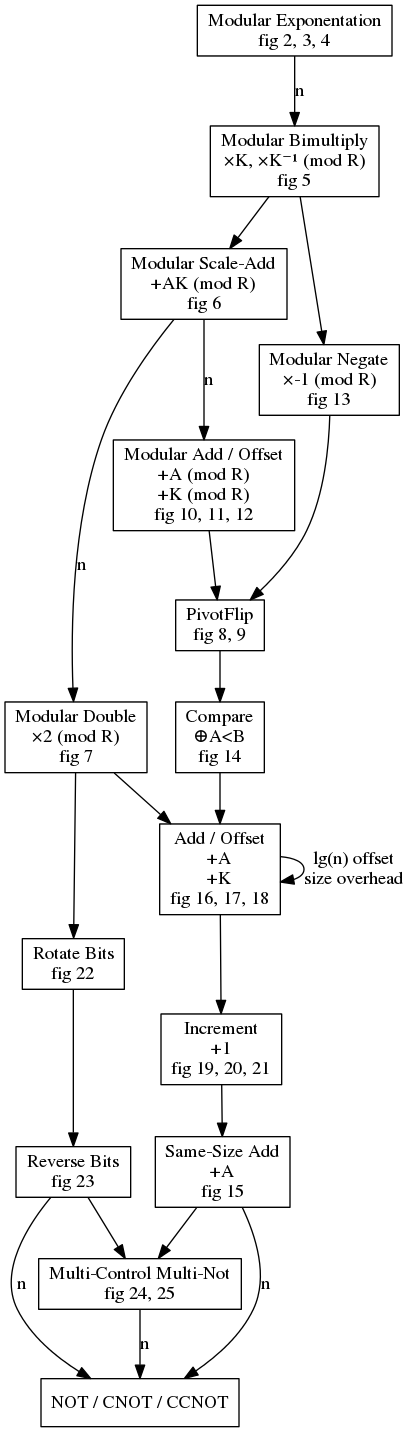
\includegraphics[height=17.3cm]{assets/dependencies.png}
  \caption{\em
    Meta-figure showing simplified dependencies between constructions, from period finding to constant-size gates.
    Edge labels indicate which constructions use their dependencies more than a constant number of times.
  }
  \label{fig:dependencies}
\end{figure}


\section{Conclusion} \label{sec:conclusion}

We presented Toffoli-based arithmetic circuits that reduce the smallest known number of qubits required to perform Shor's algorithm by 1, and allowed an additional $n-1$ qubits to be dirty.

\bibliographystyle{plain}
\bibliography{citations}

\end{document}
